\documentclass[11pt]{article}
\usepackage[T1]{fontenc}
\usepackage[utf8]{inputenc}
\usepackage{lmodern,microtype}
\usepackage[a4paper,margin=27mm,headheight=14pt]{geometry}
\usepackage{amsmath,amssymb,amsthm,mathtools}
\usepackage{booktabs,array,longtable,enumitem,graphicx,xcolor}
\usepackage{fancyhdr,needspace,xurl}
\usepackage[colorlinks=true,linkcolor=blue!45!black,citecolor=green!35!black,urlcolor=blue!50!black]{hyperref}
\usepackage[nameinlink,noabbrev]{cleveref}
\hypersetup{pdftitle={Optimized Superexponential van der Waerden Bounds and Robust Colorings},pdfauthor={ChatGPT, prepared for Vladimir Reshetnikov and the ProveIt project},pdfsubject={A quantitative refinement of the OpenAI Math family 160 construction}}
\setlength{\emergencystretch}{3em}
\setlist{itemsep=3pt,topsep=5pt}
\pagestyle{fancy}
\fancyhf{}
\fancyhead[L]{\small Optimized van der Waerden bounds}
\fancyhead[R]{\small Research report, 7 October 2026}
\fancyfoot[C]{\thepage}
\renewcommand{\headrulewidth}{0.3pt}
\numberwithin{equation}{section}
\newtheorem{theorem}{Theorem}[section]
\newtheorem{lemma}[theorem]{Lemma}
\newtheorem{proposition}[theorem]{Proposition}
\newtheorem{corollary}[theorem]{Corollary}
\newtheorem{definition}[theorem]{Definition}
\theoremstyle{remark}
\newtheorem{remark}[theorem]{Remark}
\newtheorem{question}[theorem]{Research question}
\newcommand{\N}{\mathbb N}
\newcommand{\Z}{\mathbb Z}
\newcommand{\R}{\mathbb R}
\newcommand{\T}{\mathbb T}
\newcommand{\E}{\mathbb E}
\newcommand{\Prb}{\mathbb P}
\newcommand{\cL}{\mathcal L}
\newcommand{\cK}{\mathcal K}
\newcommand{\cE}{\mathcal E}
\DeclareMathOperator{\dist}{dist}
\DeclareMathOperator{\lcm}{lcm}
\newcommand{\fl}[1]{\left\lfloor #1\right\rfloor}
\newcommand{\cl}[1]{\left\lceil #1\right\rceil}
\newcommand{\norm}[1]{\left\lVert #1\right\rVert}
\newcommand{\abs}[1]{\left\lvert #1\right\rvert}
\newcommand{\one}{\mathbf 1}
\newcommand{\oldrepo}{\texttt{openai/math}}
\newcommand{\newrepo}{\texttt{VladimirReshetnikov/ProveIt}}
\title{\bfseries Optimized Superexponential\newline van der Waerden Bounds\newline and Robust Colorings}
\author{A research report prepared for Vladimir Reshetnikov\\and the ProveIt project\\\small Developed with ChatGPT; ordinary mathematical proofs}
\date{7 October 2026}
\begin{document}
\maketitle
\begin{abstract}
We refine the cyclic construction in OpenAI Math family 160,
\emph{Quantitative Superexponential Bounds for van der Waerden Numbers}.
For absolute constants \(C,K>0\) and every integer \(k\ge K\), we prove
\[
 \log W_2(k)>
 \frac{k}{24}\bigl(\log k-5\log\log k\bigr)-Ck .
\]
The construction supplies more than nonmonochromaticity: every \(k\)-term
progression differs from every constant coloring in at least
\(\fl{b k^{2/3}(\log k)^{5/3}}\) positions, for an absolute \(b>0\).
A direct three-color version has leading coefficient \(1/18\).
Combining the two cyclic constructions gives a uniform all-color
bound with an exactly optimized binary--ternary coefficient.
The improvements come from a two-point norm-band bound, balancing
the light positions left outside heavy blocks, an elementary estimate
for the small-prime dilation, and a joint optimization of two distinct
signature costs.
We give the entire ordinary mathematical argument, including the
geometric and probabilistic ingredients inherited from the source.
This is a quantitative strengthening of that repository result, not a
new claim to have first resolved the underlying superexponential-growth
problem. No Lean formalization of the strengthened statements is claimed.
\end{abstract}

\section{Results, provenance, and the selected research problem}
\label{sec:results}

\subsection{What is being estimated}

Write \(W_r(k)\) for the least integer \(n\) such that every coloring of
\([n]=\{1,\ldots,n\}\) with at most \(r\) colors has a monochromatic
arithmetic progression of length \(k\) and positive common difference.
Unless a base is displayed, logarithms are natural. All asymptotic
statements below concern \(k\to\infty\).

For a coloring \(c\) and a \(k\)-term progression \(P=(x_j)_{j<k}\),
define its distance from monochromaticity by
\begin{equation}\label{eq:distance}
 d_{\rm mono}(c,P)
 =\min_b \#\{j<k:c(x_j)\ne b\}
 =k-\max_b\#\{j<k:c(x_j)=b\}.
\end{equation}
Thus \(d_{\rm mono}(c,P)\ge t\) says that at least \(t\) positions
must be recolored to make \(P\) monochromatic. For two colors, it says
that each color appears at least \(t\) times. For more colors it is a
statement about distance from \emph{each constant word}; it does not
say that every available color occurs.

\begin{theorem}[Two-color bound with robustness]\label{thm:main-two}
There are absolute constants \(C,b>0\) and an integer \(K\) such that,
for every integer \(k\ge K\), there is a cyclic group \(\Z/N_2\Z\) and
a two-coloring \(c\) satisfying
\begin{align}
 \log N_2&\ge
 \frac{k}{24}\bigl(\log k-5\log\log k\bigr)-Ck,
 \label{eq:main-two-size}\\
 d_{\rm mono}(c,P)&\ge
 \fl{b k^{2/3}(\log k)^{5/3}}
 \label{eq:main-distance}
\end{align}
for every nonzero-step \(k\)-term cyclic progression \(P\).
The same robustness holds on an integer interval of length
\((k-1)N_2\). In particular,
\[
 W_2(k)>(k-1)
 \exp\!\left\{\frac{k}{24}
       \bigl(\log k-5\log\log k\bigr)-Ck\right\},
 \qquad
 \liminf_{k\to\infty}\frac{\log W_2(k)}{k\log k}\ge\frac1{24}.
\]
\end{theorem}

The loss \(5k\log\log k/24\) is part of the proved bound. Its optimality
is not asserted. Neither \(C\) nor the numerical onset \(K\) is optimized;
the proof fixes them by explicit inequalities between absolute
constants and elementary functions.

\begin{theorem}[Uniform palette improvement]\label{thm:main-many}
For an integer \(r\ge2\), set
\begin{equation}\label{eq:palette-coefficient}
 m=\fl{\log_2 r},\qquad
 e(r)=
 \begin{cases}
 1,&r\ge3\cdot2^{m-1},\\
 0,&r<3\cdot2^{m-1},
 \end{cases}
 \qquad
 \Lambda(r)=\frac{m}{24}+\frac{e(r)}{72}.
\end{equation}
There are absolute \(C,b,K>0\), independent of \(r\), such that
for all integers \(k\ge K\) and \(r\ge2\),
\begin{equation}\label{eq:main-many}
 W_r(k)>(k-1)\exp\!\left\{
 \Lambda(r)k\bigl(\log k-5\log\log k\bigr)-Cmk
 \right\}.
\end{equation}
There is an \(r\)-coloring of an interval at least this long for which
every \(k\)-term progression has distance at least the quantity in
\eqref{eq:main-distance} from every monochromatic word.
\end{theorem}

The coefficient has a small but exact palette effect:
\begin{center}
\begin{tabular}{@{}c c c@{}}
\toprule
Available colors \(r\)&Digits used&\(\Lambda(r)\)\\
\midrule
2&one binary&\(1/24\)\\
3&one ternary&\(1/18\)\\
4--5&two binary&\(1/12\)\\
6--7&one binary, one ternary&\(7/72\)\\
8--11&three binary&\(1/8\)\\
12--15&two binary, one ternary&\(5/36\)\\
\bottomrule
\end{tabular}
\end{center}
The uniformity in \(r\) comes from constructing just two fixed
palettes before taking digit products.

\subsection{Repository review and choice of direction}

The review was anchored to the public OpenAI release commit
\href{https://github.com/openai/math/commit/adc7f1241b42e322a6451854ab7e4b4c146bf78a}{\texttt{adc7f1241b42}}
(6 October 2026) and the ProveIt checkpoint
\href{https://github.com/VladimirReshetnikov/ProveIt/commit/bbde2b873b2dc7b48af1730926452bdda18bf9c8}{\texttt{bbde2b873b2d}}
(7 October 2026). The source inventory includes the full commit identifiers.
The OpenAI catalog describes 722 manuscripts in 372 families and
explicitly distinguishes different verification stages
\cite{openaiReadme,openaiContents}.
The review here is a targeted comparison of the arithmetic-progression
families and the active ProveIt Ramsey work, rather than a certification
of every result in either repository.

\begin{center}
\small
\begin{tabular}{@{}>{\raggedright\arraybackslash}p{.19\textwidth}>{\raggedright\arraybackslash}p{.35\textwidth}>{\raggedright\arraybackslash}p{.37\textwidth}@{}}
\toprule
Source&Relevant result or status&Consequence for this project\\
\midrule
OpenAI family 159&
Claims \(r_k(N)\le C_kN\) \(\exp[-c_k(\log N)^{\varepsilon_k}]\);
the described comparator emphasizes the reciprocal-sum consequence
\cite{openai159,openai159Scope}.&
A strong density-theorem overlap, but its paper already contains
several natural weighted and coloring consequences.\\
\addlinespace
OpenAI family 160&
Proves the displayed bound
\(W_r(k)>k^{10^{-5}k\lfloor\log_2r\rfloor}\);
the scope file records this formalized endpoint
\cite{openai160,openai160Scope}.&
An elementary, sufficiently explicit construction whose quantitative
losses can be inspected and improved.\\
\addlinespace
ProveIt Ramsey&
The inspected checkpoint records 113 of 120 exact Gowers statements,
with seven open; recent intake includes sharp hereditary-energy
results and failures of universal lifting interfaces
\cite{proveitStatus,proveitIntake}.&
Motivates exact bookkeeping, careful quantifiers, and a complete
proof boundary. A lower-bound project avoids duplicating the large
existing collection of local upper-bound refinements.\\
\bottomrule
\end{tabular}
\end{center}

The same ProveIt status file records 137 vendored OpenAI Lean modules
in its build, an exact qualitative Szemer\'edi statement proved by a
route distinct from the original Gowers argument, and completed
Freiman and Balog--Szemer\'edi interfaces using OpenAI modules
\cite{proveitStatus}. Thus the intersection is already concrete:
arithmetic-progression research is being assembled with explicit
theorem interfaces and a record of which claims are checked.
These are statements of the inspected repository checkpoint; this
report did not independently run that Lean build.

The direct research question selected was:
\emph{how far can the coefficient in family 160 be increased while
retaining a fully justified growing-dimensional construction, and can
the resulting colorings be made quantitatively resistant to
monochromaticity?}
The answer is \cref{thm:main-two,thm:main-many}.

\subsection{The precise increment over prior work}

The underlying cyclic embedding, adaptive mesh, anchored counting
argument, local lemma, and norm-indexed perturbation are due to
OpenAI's source manuscript \cite{openai160}.
They are reconstructed below with the changed hypotheses visible.
The new quantitative steps established in this report are:
\begin{enumerate}
 \item A norm-band key has at most \emph{two} occurrences on a
 progression, improving the source's upper bound of four.
 \item The local lemma simultaneously balances residual light sets
 after heavy blocks are removed. This yields a
 \((1/2-o(1))\)-balanced-or-affine dichotomy in two colors; balancing
 the entire light set alone would not justify this conclusion.
 \item The short-period cutoff can be chosen of order
 \(D(\log k)^3\) at balance accuracy \(1/\log k\), and
 \(\log\lambda=O(D(\log k)^3)\) follows from an elementary prime-count
 estimate. This replaces the much larger power-scale cutoff in
 the source and avoids an unnecessary logarithmic loss.
 \item Global label entropy and quadratic-signature entropy are
 optimized together. Their balance gives
 \(D\asymp k^{1/3}(\log k)^{-2/3}\) and
 \(p\asymp k^{-1/3}(\log k)^{5/3}\), and hence the coefficient \(1/24\).
 \item A bounded-variable lower-tail argument and an exception-set
 count give the robustness estimate. A three-color construction and
 an optimized mixed-radix product give \(\Lambda(r)\).
\end{enumerate}
The finite periodic extension factor \(k-1\) is an existing observation,
used explicitly by Campos--Fox--Schildkraut
\cite[Lemma 2]{camposFoxSchildkraut2026}; it is credited and proved
again in the robust setting.

These are quantitative improvements to a result already present in
the release, rather than a second claim of priority for
superexponential growth. A bounded search of the inspected ProveIt
Ramsey material and then-current incoming reports found no report
containing these refinements. That observation is not a proof of
global bibliographic novelty.

\subsection{Comparison with the contemporary literature}

Fox and Hunter prove three-color superexponential growth, including
\(W_3(k)>2^{k\log^*k/4}\) for large \(k\)
\cite[Theorem 1]{foxHunter2026}.
Campos, Fox, and Schildkraut prove
\(W_2(k)\ge(1-o(1))k2^{k-1}\)
\cite[Theorem 1]{camposFoxSchildkraut2026}.
The source paper \cite{openai160} subsequently supplies the
two-color \(k^{ck}\) construction used here.
The displayed two-color leading coefficient in this report is
\((1/24)/10^{-5}=12500/3\) times the displayed source coefficient.
This compares asymptotic exponents, not practical lower bounds for
small numerical values of \(k\).

Our uniform all-color bound is useful down to two and three colors.
It is not the strongest known estimate in every growing-color regime.
For each fixed \(0<\varepsilon<1\), Fox--Hunter
\cite[Theorem 2]{foxHunter2026} prove
\[
 W_r(k)\ge r^{(1-\varepsilon)k\log k}
 \quad\text{when }\
 k\ge k_0(\varepsilon),\qquad
 r\ge(\log k)^{3/\varepsilon}.
\]
For example, their choice \(\varepsilon=1/2\) is stronger than our
leading coefficient once its hypotheses apply.
Both bounds can simply be retained in the appropriate regime.

\subsection{Proof conventions and status}

All probabilistic spaces used below are finite. Equality at every mesh
boundary is handled by a fixed half-open convention; key identities
retain their actual labels and are never renamed when events are
identified. Constants denoted \(C_0,C_1,\ldots\) are absolute, and
subscripts such as \(C_A\) indicate dependence on a previously fixed
absolute choice. The choice order is
\[
  \text{geometric constants}\quad\longrightarrow\quad A
  \quad\longrightarrow\quad B\quad\longrightarrow\quad C
  \quad\longrightarrow\quad K .
\]
The proof of the strengthened results is an ordinary mathematical
proof presented in this report. Source scope files are not a substitute
for running a prover; no build of the OpenAI or ProveIt Lean library
was performed here. The exact-arithmetic companion checks finite
identities and the palette optimization, and is not represented as a
certificate of the asymptotic existence theorem.

\clearpage
\tableofcontents
\clearpage
\section{Cyclic geometry and an economical short-period dilation}
\label{sec:geometry}

Fix a palette size \(s\in\{2,3\}\). The same estimates will work for
both choices. Set
\begin{equation}\label{eq:parameters}
\begin{gathered}
 L=\log k,\qquad \zeta=L^{-1},\qquad
 D=\cl{k^{1/3}L^{-2/3}},\qquad M=\cl{k^{3/4}},\\
 h_0=\cl{A D L^3},\qquad H=k^{-2},\qquad
 \eta=\frac{\zeta}{100D},\qquad
 p=B k^{-1/3}L^{5/3}.
\end{gathered}
\end{equation}
Here \(A\) and then \(B\) are sufficiently large absolute constants.
They will be fixed in the local-lemma and perturbation arguments.
All assertions in this section hold for sufficiently large \(k\)
after those constants are fixed. In particular,
\[
 1\ll D<h_0<2M<k,\qquad p<1/2,\qquad 2kH<1.
\]
The relatively generous choice \(M=k^{3/4}+O(1)\) separates the
global local-lemma tests from the signature costs.

\subsection{The elementary prime estimates actually needed}

\begin{lemma}\label{lem:prime-estimates}
For some absolute \(C_\pi\), the number \(\pi(x)\) of primes at most
\(x\) satisfies \(\pi(x)\le C_\pi x/\log x\) for \(x\ge2\).
For every sufficiently large integer \(k\), a prime \(P\) exists with
\(k<P\le2k^2\).
\end{lemma}

\begin{proof}
Every prime in \((n,2n]\) divides \(\binom{2n}{n}\), and
\(\binom{2n}{n}\le4^n\). Therefore
\(\sum_{n<\ell\le2n,\ \ell\ {\rm prime}}\log\ell\le2n\log2\).
Summing at powers of two proves
\(\vartheta(x)=\sum_{\ell\le x}\log\ell\le C_\vartheta x\)
with an absolute constant. Primes exceeding \(\sqrt{x}\) each
contribute at least \(\frac12\log x\), so
\[
 \pi(x)\le \sqrt{x}+\frac{2\vartheta(x)}{\log x}
 \le C_\pi \frac{x}{\log x},
\]
after increasing the constant to cover the bounded initial range.
This is the elementary Chebyshev upper estimate.

For the second assertion put \(n=k^2\). The factorial formula gives
\[
 v_\ell\binom{2n}{n}
 =\sum_{a\ge1}
 \left(\fl{\frac{2n}{\ell^a}}-2\fl{\frac n{\ell^a}}\right)
 \le\fl{\log_\ell(2n)} .
\]
If all prime divisors were at most \(k\), then
\(\binom{2n}{n}\le(2n)^k\).
But the largest binomial coefficient is at least \(4^n/(2n+1)\),
which exceeds \((2n)^k\) for \(n=k^2\) and large \(k\).
A prime divisor exceeding \(k\) therefore exists, and it is at most
\(2n\).
\end{proof}

Choose the dilation
\begin{equation}\label{eq:dilation}
 \lambda=
 \prod_{\substack{\ell\le h_0\\\ell\ {\rm prime}}}
 \ell^{\fl{\log(2M)/\log\ell}} .
\end{equation}

\begin{lemma}[Period removal and dilation cost]\label{lem:dilation}
If \(1\le h\le2M\), every primary factor of \(h\) at a prime at most
\(h_0\) divides \(\lambda\). Consequently
\[
 h\le h_0\ \Longrightarrow\ h\mid\lambda,\qquad
 \frac{h}{\gcd(h,\lambda t)}\in\{1\}\cup(h_0,\infty)
 \quad(t\in\Z).
\]
For the choices \eqref{eq:parameters},
\begin{equation}\label{eq:dilation-cost}
 \log\lambda=O(h_0),\qquad
 D\log\lambda=O_A(k^{2/3}L^{5/3}).
\end{equation}
\end{lemma}

\begin{proof}
If \(\ell^a\mid h\le2M\), then
\(a\le\fl{\log(2M)/\log\ell}\).
After division by \(\gcd(h,\lambda t)\), all remaining prime
divisors therefore exceed \(h_0\). This proves the period statements.
Every factor of the product \eqref{eq:dilation} is at most \(2M\).
By \cref{lem:prime-estimates},
\[
 \log\lambda\le\pi(h_0)\log(2M)
 \le C_\pi h_0\frac{\log(2M)}{\log h_0}=O(h_0),
\]
since the ratio of logarithms tends to \(9/4\).
Finally \(D h_0=O_A(D^2L^3)=O_A(k^{2/3}L^{5/3})\).
\end{proof}

The bound \(\log\lambda=O(h_0)\), rather than the cruder
\(O(h_0\log M)\), is responsible for the improved logarithmic correction
in the final theorem. No prime number theorem or primes in short
intervals is required.

\subsection{The cyclic embedding and its scales}

Let
\begin{equation}\label{eq:target}
 a_s=\frac{s-1}{12s},\qquad
 Q_s(k)=a_s k(L-5\log L)-Ck,
\end{equation}
where \(C>0\) will be fixed last among the constants.
Choose a prime \(P\) from \cref{lem:prime-estimates}, and let \(q\)
be the smallest positive power of \(P\) satisfying
\(q\ge\exp(Q_s(k)/D)\). Then
\begin{equation}\label{eq:q-rounding}
 Q_s(k)\le D\log q\le Q_s(k)+D\log(2k^2),
 \qquad
 \log q=O(k^{2/3}L^{5/3}).
\end{equation}
The rounding error \(D\log(2k^2)\) is \(o(k)\).
For large \(k\), \(P>k>h_0\), so \(\lambda\) is invertible modulo
every power of \(q\).

Put \(N=q^D\), \(G=\Z/N\Z\), and \(\T=\R/\Z\). Use the homomorphisms
\begin{equation}\label{eq:coordinates}
 x_i(n)=n/q^i\pmod1,\qquad
 y_i(n)=\lambda n/q^i\pmod1,\qquad 1\le i\le D.
\end{equation}
We denote the representatives of the two vectors by
\(\widehat{x}(n)\in[0,1)^D\) and
\(\widetilde{y}(n)\in[-1/2,1/2)^D\).
Every nonzero element of \(G\) has order at least \(P>k\).
Thus a nonzero-step \(k\)-term cyclic progression always has distinct
terms.

Set
\[
 H_x=H/\lambda,\qquad \alpha=q^{-(D+1)},\qquad
 \rho(Y)=\dist_\T(Y,1/2).
\]
The function \(\rho\) is \(1\)-Lipschitz and takes values in
\([0,1/2]\).
Partition \([0,1)\) into intervals of length \(H_x\); this gives a
partition \(U\) with exactly \(k^2\lambda\) intervals.
For the second coordinate system put
\begin{equation}\label{eq:adaptive-mesh}
 R=\log(1+(2\alpha)^{-1}),\quad
 J_0=\cl{k^2R},\quad
 a_j=\alpha\bigl(e^{jR/J_0}-1\bigr)\quad(0\le j\le J_0).
\end{equation}
The partition \(V\) of \([-1/2,1/2)\) consists of
\[
 [-1/2+a_j,-1/2+a_{j+1}),\quad
 [1/2-a_{j+1},1/2-a_j)
 \qquad(0\le j<J_0).
\]
In particular, zero is assigned to the interval on its right, and the
cut is assigned to the interval beginning at \(-1/2\).
All interval labels retain the identities and locations of their
intervals. Write
\begin{equation}\label{eq:labels}
 \cL=U^D\times V^D,\qquad
 L(n)=\bigl((U(x_i(n)))_{i=1}^D,(V(y_i(n)))_{i=1}^D\bigr).
\end{equation}
For arbitrary \(X,Y\in\T^D\), the notation \(L(X,Y)\) has the analogous
meaning.

\begin{lemma}[Adaptive-mesh estimates]\label{lem:mesh}
For \(I\in V\), \(Y\in\overline I\), and sufficiently large \(k\),
\begin{equation}\label{eq:mesh-width}
 \frac H4(\rho(Y)+\alpha)\le |I|
 \le2H(\rho(Y)+\alpha)\le2H,\qquad |V|=O(k^3L).
\end{equation}
If \(w=|I|\) and
\(\mathcal N(I)=\{Y:\dist_\T(Y,\overline I)\le w\}\), every
mesh interval whose closure meets \(\mathcal N(I)\) has length at
least \(w/16\). There are at most \(49\) mesh endpoints in
\(\mathcal N(I)\).

Define \(V_\eta(Y)=V(Y)\) when \(\rho(Y)\ge\eta\), and
\(V_\eta(Y)=*\) otherwise. On any circle arc of length at most \(4H\),
this function has at most \(C_0D/\zeta\) breakpoints, with an absolute
\(C_0\). At a breakpoint the output is fixed by the stated conventions.
\end{lemma}

\begin{proof}
Write \(\theta=R/J_0\). For large \(k\), \(H/2\le\theta\le H\).
On a mesh interval, \(\rho(Y)+\alpha\) ranges between
\(b=\alpha e^{j\theta}\) and \(be^\theta\), whereas its length is
\(b(e^\theta-1)\). The inequalities
\[
 \theta/2\le1-e^{-\theta}
 \le\frac{|I|}{\rho(Y)+\alpha}
 \le e^\theta-1\le2\theta
\]
give \eqref{eq:mesh-width}. Since
\(R\le(D+1)\log q=O(kL)\), we have \(2J_0=O(k^3L)\).

Fix \(Y_0\in\overline I\) and \(r_0=\rho(Y_0)+\alpha\).
A point in \(\mathcal N(I)\) has distance at most \(2w\) from \(Y_0\).
Therefore its value of \(\rho+\alpha\) is at least
\(r_0-2w\ge(1-4H)r_0\ge r_0/2\).
Applying the lower width estimate to a point of
\(\overline J\cap\mathcal N(I)\) gives
\(|J|\ge Hr_0/8\ge w/16\).
The arc \(\mathcal N(I)\) has length \(3w<1\).
Consecutive endpoints in it enclose a complete mesh interval of
length at least \(w/16\), so their number is at most \(49\).

On an arc of length \(4H\), the portion with \(\rho\ge\eta\) has at
most two components. Consecutive mesh endpoints within a component
are separated by at least \(H\eta/4\). There are at most
\(16/\eta+2\) such endpoints, and at most two more threshold points
where \(\rho=\eta\). As \(\eta=\zeta/(100D)\), this is
\(O(D/\zeta)\). The other portions have the single dummy output.
\end{proof}

\subsection{Small boxes force real affinity}

\begin{lemma}[Affinity on the visits to one box]\label{lem:box-affine}
Let \(z_j=a+jb\) in \(\T^e\), \(0\le j<k\), and let \(J\) be a
set of indices. Suppose the chosen real representatives \(Z_j\),
\(j\in J\), all lie in one box of coordinate widths at most \(2H\).
If \(2kH<1\), there are \(A_0,B_0\in\R^e\) such that
\(Z_j=A_0+jB_0\) for \(j\in J\).
\end{lemma}

\begin{proof}
For \(j_1<j_2<j_3\) in \(J\), the vector
\[
 (j_3-j_2)(Z_{j_2}-Z_{j_1})
 -(j_2-j_1)(Z_{j_3}-Z_{j_2})
\]
is integral because it is zero modulo \(\Z^e\).
Each coordinate has absolute value at most
\(2H(j_3-j_1)<1\), so the vector is zero.
Interpolation between the extreme visits now gives the result.
The cases \(|J|\le2\) require only direct interpolation.
\end{proof}

Fix a cyclic progression \(n_j=n_0+jd\), \(d\ne0\).
A label is \emph{heavy} if it occurs more than \(k/M\) times on this
whole progression, and \emph{light} otherwise. Positions are
designated by their labels; the designations do not change on passing
to a block.

\begin{lemma}[A heavy label determines a rational return]\label{lem:return}
If a heavy label occurs \(m_*>k/M\) times, there are
\(1\le h\le2M\), \(t\in\{0,\ldots,h-1\}^D\), and \(u,v\in\R^D\)
such that
\begin{align}
 x(n_j)&=x(n_0)+\frac jh(t+u),&
 y(n_j)&=y(n_0)+\frac jh(\lambda t+v)
 \quad\text{in }\T^D,\label{eq:return-path}\\
 |u_i|&\le\frac{2MH_x}{k},&
 |v_i|&\le\frac{4MH}{k},\qquad v=\lambda u.
 \label{eq:return-drift}
\end{align}
Moreover \(\gcd(t_1,\ldots,t_D,h)=1\).
Incongruent indices modulo \(h\) have different full labels.
For every heavy position \(j_*\), not just one of the initially chosen
label, the stronger estimate
\begin{equation}\label{eq:heavy-relative}
 |v_i|\le\frac{2M}{k}\,|V(y_i(n_{j_*}))|
\end{equation}
holds.
\end{lemma}

\begin{proof}
Let \(J\) be the occurrences of the chosen heavy label, and let \(h\)
be its smallest positive gap, attained at \(j'\) and \(j'+h\).
If \(j_-=\min J\), \(j_+=\max J\), then
\[
 h\le\frac{j_+-j_-}{m_*-1}\le2M,\qquad
 m_*-1\ge k/(2M).
 \]
Apply \cref{lem:box-affine} to both coordinate systems together.
The real differences \(u,v\) between these two closest visits are
\(h/(j_+-j_-)\) times the endpoint differences. Their coordinate
widths are \(H_x,2H\), which proves \eqref{eq:return-drift}.
Since \(v-\lambda u\) is integral and has coordinates of absolute
value at most \(6MH/k<1\), it is zero.
The relation \(h x(d)=u\) in the torus gives an integral vector
\(t'=h\widehat{x}(d)-u\); reduce it modulo \(h\) to obtain \(t\).
This proves \eqref{eq:return-path}.

If an integer \(e>1\) divides \(h\) and every \(t_i\), the point
at \(j'+h/e\) is represented by the convex combination with weight
\(1/e\) of the representatives at \(j'\) and \(j'+h\).
It is in the same product of half-open intervals, contradicting the
minimal gap \(h\). Thus the gcd is one.
For indices incongruent modulo \(h\), the rational displacement has
some coordinate at circle distance at least \(1/h\) from zero.
The drift subtracts at most \(2MH_x/h\).
The resulting distance is at least
\((1-2MH)/(2M)>H_x\), so their \(U\)-labels differ.

Finally take any heavy label, of multiplicity \(m'>k/M\), with
extreme visits \(j_-,j_+\). All its visits are in one residue class
modulo \(h\), so \(j_+-j_-=a h\), where \(a\ge m'-1\) and \(a<k/h\).
Let \(L_i=|V(y_i(n_{j_*}))|\). The real endpoint difference
\(\Delta_i\) has absolute value at most \(L_i\) and is congruent to
\(av_i\) modulo one. The bounds
\[
 |av_i|\le4MH/h,\qquad
 |\Delta_i-av_i|\le2H+4MH/h<1
\]
show that \(\Delta_i=av_i\).
Dividing by \(a\ge m'-1\ge k/(2M)\) proves
\eqref{eq:heavy-relative}.
\end{proof}

\begin{lemma}[Short returns have one global lift]\label{lem:short}
In \cref{lem:return}, if \(h\le h_0\), then
\(\widetilde y(n_j)=A_0+jB_0\) in \(\R^D\) for all \(0\le j<k\).
\end{lemma}

\begin{proof}
Since \(h\mid\lambda\), the rational part of the second path
vanishes in the torus. Its real drift step is \(w=v/h\), with
\(k|w_i|\le4MH/h<1/2\).
Also \(w_i\in q^{-i}\Z\), since \(w_i\) represents \(y_i(d)\);
if it is nonzero then \(|w_i|\ge q^{-D}\ge\alpha\).

If the centered representatives fail to follow the single real
segment \(\widetilde y_i(n_0)+\tau w_i\), that segment meets a
representative cut in some coordinate with \(w_i\ne0\).
Every sample then has \(\rho(y_i(n_j))\le k|w_i|\), including
endpoint cut hits. By \eqref{eq:mesh-width},
\[
 |V(y_i(n_j))|\le2H(k+1)|w_i|<|w_i|.
\]
Yet any two samples have circle separation
\(|j-j'|\,|w_i|\ge |w_i|\), since their total motion is less than
\(1/2\). No two can share a \(V\)-interval. This contradicts the
heavy label, and proves the claim.
\end{proof}

\section{Pattern counts and a nearly uniform outer coloring}
\label{sec:outer}

\subsection{Counting comparisons, with equality retained}

\begin{lemma}[Arrangement count]\label{lem:arrangement}
The joint signs, including zero signs, of \(u\) affine functions on
\(\R^e\) have at most
\begin{equation}\label{eq:arrangement}
 \sum_{d=0}^e\binom ud\sum_{j=0}^{e-d}\binom uj
 \le(e+1)^2(u+1)^e
\end{equation}
realized values. Restricting the parameter domain does not increase
this count.
\end{lemma}

\begin{proof}
The strict regions of \(u\) hyperplanes in dimension \(e\) number at
most \(\sum_{j=0}^e\binom uj\). Add the hyperplanes one at a time:
a new hyperplane splits no more regions than the number of regions
in its induced arrangement of dimension \(e-1\). Induction and
Pascal's identity prove the bound.
For a sign pattern with zero signs, select \(d\) independent zero
equations defining their common affine intersection. There are at
most \(\binom ud\) choices. On that intersection count strict regions
in dimension \(e-d\); all equations vanishing identically there have
forced zero signs. Sum over \(d\). The final estimate follows by
bounding every binomial product by \((u+1)^e\).
\end{proof}

This elementary form of the standard arrangement bound
\cite{stanley2007} keeps exact boundary events visible.

\begin{lemma}[Global label entropy]\label{lem:global}
Let \(T_{\rm glob}\) be the number of literal label words
\((L(n_j))_{j<k}\) of nonzero-step cyclic progressions. Then
\begin{equation}\label{eq:global-entropy}
 \log T_{\rm glob}
 =O\!\left(D(\log k+\log\lambda)\right)
 =O_A(k^{2/3}L^{5/3}).
\end{equation}
\end{lemma}

\begin{proof}
For a circle partition with \(F\) endpoints, freely vary a scalar
start and step \(a,b\in[0,1)\). The labels of
\((a+jb)\bmod1\), \(j<k\), are determined by comparisons of \(a+jb\)
with all lifts \(\tau+z\) of endpoints, where \(-1\le z\le k\).
At most \(3k^2F\) affine lines in the parameters \((a,b)\) suffice.
By \cref{lem:arrangement}, there are at most
\(9(3k^2F+1)^2\) scalar words.

Apply this separately to all \(2D\) coordinates. Letting their starts
and steps vary independently only enlarges the possible set.
We may take \(F=|U|+|V|=k^2\lambda+O(k^3L)\), so
\[
 T_{\rm glob}\le[9(3k^2F+1)^2]^{2D}.
\]
Now use \cref{lem:dilation}. The identity of every interval, not just
its rank among the visits, is preserved in this count.
\end{proof}

\subsection{Eligible blocks and counting through one fixed label}

Fix \(h_0<h\le2M\) and \(t\in\{0,\ldots,h-1\}^D\).
In the second coordinate system define
\[
 s_i=\frac{h}{\gcd(h,\lambda t_i)}.
\]
A coordinate is \emph{stationary} if \(s_i=1\), and \emph{rotating}
otherwise. By \cref{lem:dilation}, a rotating coordinate has \(s_i>h_0\).
Stationary refers only to its rational motion; a real drift is allowed.

\begin{definition}\label{def:eligible}
Consider paths, in the torus,
\[
 X_z=x+\frac zh(t+u),\qquad
 Y_z=y+\frac zh(\lambda t+v),\qquad 0\le z<h,
\]
where \(x,y\in\T^D\) and \(u,v\in\R^D\).
A position is \emph{regular} when
\(\rho(Y_{z,i})\ge\eta\) in every rotating coordinate.
Record \(L(X_z,Y_z)\) at a regular position and a dummy symbol at
every other position.
The resulting literal word is \emph{eligible} for \(h,t\) if it has
a realization satisfying all of the following:
\begin{enumerate}
 \item at least \(h/2\) positions are regular, and their full labels
       are pairwise distinct;
 \item \(|u_i|\le H_x\) in every coordinate and \(|v_i|\le H\)
       in each rotating coordinate;
 \item in each stationary coordinate,
       \(|v_i|\le |V(Y_{z,i})|\) at every regular position.
\end{enumerate}
\end{definition}

Only the recorded word and \(h,t\) are counted; its potentially many
real realizations do not give extra events.

\begin{lemma}[Anchored local count]\label{lem:local}
There is an absolute constant \(C_1\) such that for any full label
\(\beta\) and \(h_0<h\le2M\), the number of pairs consisting of \(t\)
and an eligible pattern for \(h,t\) containing \(\beta\) is at most
\begin{equation}\label{eq:local-count}
 \left(\frac{C_1 D h}{\zeta}\right)^{6D}.
\end{equation}
The constant is independent of \(q,\lambda\), and the widths of the
intervals in \(\beta\).
\end{lemma}

\begin{proof}
Fix \(t\) and an anchor index \(z_0\) recording \(\beta\).
In any scalar coordinate re-anchor the representative at \(z_0\).
Its value at \(z\) before reducing modulo one is
\[
 a+\tau_z+\frac{z-z_0}{h}b,
\]
where \(\tau_z\) is fixed, \(a\) belongs to the interval in \(\beta\),
and \(b\) is the appropriate drift.
We retain only the restrictions on \(a,b\) imposed at the anchor.
For a first coordinate the total target range has length at most
\(3H_x\), hence meets at most four lifted \(U\)-endpoints.
For a stationary second coordinate with anchor interval \(I\), the
translation is integral and \(|b|\le |I|\).
Every target lies in \(\mathcal N(I)\), meeting at most \(49\)
endpoints by \cref{lem:mesh}.
For a rotating second coordinate the target range has length at most
\(4H\), and its truncated output is determined by at most
\(C_0D/\zeta\) breakpoints.

All the enclosing ranges and breakpoint lifts are fixed before
\((a,b)\) vary. Their magnitude introduces no additional factor:
each range is shorter than one in the second system, so each
relevant circle breakpoint has at most one lift in it.
Over all \(h\) positions there are \(O(Dh/\zeta)\) comparisons in
two real parameters. Thus the scalar output has at most
\(C_2(Dh/\zeta)^2\) possibilities, including boundary outputs.
Taking the product over \(2D\) scalar coordinates determines the
dummy mask as well as the actual regular labels.
There is no separate mask to enumerate.

There are \(h^D\) choices of \(t\) and at most \(h\) choices of \(z_0\).
The resulting bound is
\[
 h^{D+1}[C_2(Dh/\zeta)^2]^{2D}
 \le(C_1Dh/\zeta)^{6D},
\]
after enlarging an absolute constant.
\end{proof}

\subsection{Residual tests: the change needed for near-uniformity}

For each realized word \(w\) and integer \(h_0<h\le2M\), divide its
first \(h\fl{k/h}\) positions into consecutive blocks of length \(h\).
Let
\begin{equation}\label{eq:residual-set}
 S(w,h)=\bigcup\{\text{full blocks containing no heavy position of }w\}.
\end{equation}
Every position in this set is light. Crucially, \(S(w,h)\) is determined
by \(w,h\), rather than being an arbitrary subset of the light
positions.

We impose two global kinds of tests: the set of all light positions,
and each \(S(w,h)\). A test is included only if its set has at least
\(\zeta k\) positions. For such a set \(S\), let \(w_{\max}\) be its
maximum label multiplicity. Group occurrences by label, fix their
order deterministically from the word, and distribute the list
cyclically into \(w_{\max}\) rows.
Each row has distinct labels and at least
\begin{equation}\label{eq:row-length}
 \fl{|S|/w_{\max}}\ge\zeta M-1
\end{equation}
positions. The number of row tests is at most
\(k(2M+1)T_{\rm glob}\).

The local tests are all eligible recorded patterns, tested on their
regular positions. Each also has distinct labels.
For a test of length \(l\), we require each color \(b\in\Z/s\Z\)
to occur between \((1/s-\zeta)l\) and \((1/s+\zeta)l\).

\begin{lemma}[Finite local lemma]\label{lem:lll}
Let finitely many events \(E\) have a dependency graph such that
each \(E\) is independent of the joint sigma-algebra of its
nonneighbors. If \(0<z_E<1\) and
\[
 \Prb(E)\le z_E\prod_{F\sim E}(1-z_F)
\]
for every \(E\), then all their complements have positive joint
probability.
\end{lemma}

\begin{proof}
An induction on the number of conditioned complements proves
\(\Prb(E\mid\bigcap_{F\in T}F^c)\le z_E\) whenever \(E\notin T\),
and proves that every such conditioning event has positive probability.
For the conditional estimate split \(T\) into neighbors \(T_1\) of
\(E\) and nonneighbors \(T_2\).
If \(T_1\) is empty, use independence.
Otherwise expose the complements in \(T_1\) one at a time after
conditioning on \(T_2\). The induction hypothesis gives a denominator
at least \(\prod_{F\in T_1}(1-z_F)\), while independence bounds the
numerator by \(\Prb(E)\).
The displayed hypothesis completes the induction.
Positivity follows by multiplying the conditional probabilities of
successive complements. This is the finite asymmetric local lemma
\cite{erdosLovasz1975}.
\end{proof}

\begin{proposition}[Simultaneously balanced tests]\label{prop:outer-tests}
For sufficiently large absolute \(A\), and then all sufficiently large
\(k\), there is a coloring \(c_*:\cL\to\Z/s\Z\) satisfying every
global row test and every eligible local test above, for \(s=2\)
or \(s=3\).
\end{proposition}

\begin{proof}
Color each label independently and uniformly in \(\Z/s\Z\).
For a fixed color its count on \(l\) distinct labels is a sum of
independent Bernoulli variables of mean \(1/s\).
For a Bernoulli variable \(X\) with mean \(q\), the function
\[
 g(t)=\log(1-q+qe^t)-qt
\]
has \(g(0)=g'(0)=0\) and \(g''(t)\le1/4\).
Hence \(\E e^{t(X-q)}\le e^{t^2/8}\).
Markov's inequality with \(t=4\zeta\), and the analogous negative
value, gives a two-sided tail at most \(2e^{-2\zeta^2l}\).
Union over the at most three colors bounds each bad event by
\begin{equation}\label{eq:hoeffding}
 \Prb(E)\le6e^{-2\zeta^2l(E)}.
\end{equation}

Assign \(z_E=e^{-\zeta^2l(E)/2}\).
For any one label, the total incident weight from global events is
at most
\begin{equation}\label{eq:global-weight}
 k(2M+1)T_{\rm glob}
 \exp[-\zeta^2(\zeta M-1)/2]=o(\zeta^2).
\end{equation}
Indeed its positive logarithm is \(O_A(k^{2/3}L^{5/3})+O(L)\),
whereas its negative term has order \(k^{3/4}/L^3\).
The latter grows faster.
For local events \cref{lem:local} bounds the incident weight by
\begin{equation}\label{eq:local-weight}
 \sum_{h>h_0}
 (C_1Dh/\zeta)^{6D} e^{-\zeta^2h/4}.
\end{equation}
The function \(\log(C_1Dh/\zeta)/h\) is decreasing for \(h\ge h_0\)
once \(k\) is large. At the initial point,
\[
 \frac{6D\log(C_1Dh_0/\zeta)}{h_0}
 =\left(\frac4A+o(1)\right)\zeta^2.
\]
Choose \(A\) large enough that this is at most \(\zeta^2/8\).
Then \eqref{eq:local-weight} is at most
\[
 \sum_{h>h_0} e^{-\zeta^2h/8}
 =O\!\left(\zeta^{-2}e^{-\zeta^2h_0/8}\right)
 =o(\zeta^2).
\]
These estimates also show \(\zeta^2l(E)\to\infty\) uniformly over the
included tests.

Join events sharing a label. They have the required dependency
property because the underlying label colors are independent.
For large \(k\), the total weight incident to any label is at most
\(\zeta^2/16\), so
\(\sum_{F\sim E}z_F\le\zeta^2l(E)/16\).
All weights are less than \(1/2\), and
\(\log(1-z)\ge-2z\) on that interval. Consequently
\[
 z_E\prod_{F\sim E}(1-z_F)
 \ge e^{-5\zeta^2l(E)/8}
 \ge6e^{-2\zeta^2l(E)}
 \ge\Prb(E).
\]
Apply \cref{lem:lll}, and fix one successful coloring \(c_*\).
\end{proof}

Define \(c_0(n)=c_*(L(n))\).
All randomness used for this outer coloring is now finished.

\begin{theorem}[Nearly uniform or globally affine]\label{thm:dichotomy}
For every nonzero-step cyclic progression \(n_j=n_0+jd\), either
its entire centered second-coordinate path is affine in \(\R^D\),
or, for every color \(b\in\Z/s\Z\),
\begin{align}
 \#\{j:c_0(n_j)=b\}&\ge(1/s-4\zeta)k,\label{eq:outer-each}\\
 \#\{j:c_0(n_j)\ne b\}&\ge(1-1/s-4\zeta)k.\label{eq:outer-complement}
\end{align}
\end{theorem}

\begin{proof}
If all labels are light, the global test on all \(k\) positions proves
both assertions, with \(\zeta\) in place of \(4\zeta\).
Otherwise use a heavy label to obtain \(h,t,u,v\) from
\cref{lem:return}. When \(h\le h_0\), \cref{lem:short} gives the
affine alternative.

Suppose \(h>h_0\). For a rotating coordinate, the rational part of a
full \(h\)-block visits an equally spaced \(s_i\)-point grid, each point
\(h/s_i\) times, where \(s_i>h_0\).
The actual drift has magnitude at most \(4MH/k<\eta\).
Nonregular positions in that coordinate therefore correspond to grid
points within \(2\eta\) of the cut.
An arc of length \(4\eta\) contains at most \(4\eta s_i+1\) such
grid points, including endpoints.
The nonregular fraction in a block is thus at most
\[
 D(4\eta+1/h_0)
 =\zeta/25+D/h_0\le\zeta.
\]
Distinct block indices have distinct full labels by
\cref{lem:return}. Also \(|u_i|\le H_x\) and \(|v_i|\le H\)
eventually.

Any full block containing a heavy position \(j_*\) is eligible.
To check its only remaining condition, take a stationary coordinate,
and put \(I_*=V(y_i(n_{j_*}))\), \(w_*=|I_*|\).
The circle displacement within the block is at most
\(|v_i|\le(2M/k)w_*\).
By the neighborhood estimate of \cref{lem:mesh}, every interval
visited in that block has length at least \(w_*/16\).
Since \(2M/k\le1/16\) eventually, its length is at least \(|v_i|\).
This proves eligibility even if the heavy anchor itself is nonregular.

Let \(B_*\) be the union of heavy-containing full blocks, and let
\(S=S(w,h)\) be their light complement among the full blocks.
The remaining tail has fewer than \(h\le2M\le\zeta k\) positions.
For either the indicator of one color or its complement, let its
uniform mean be \(\beta\), where \(\beta=1/s\) or \(1-1/s\).
The local tests give at least
\((\beta-\zeta)(1-\zeta)|B_*|\) successes on \(B_*\).
If \(|S|\ge\zeta k\), its row tests add
\((\beta-\zeta)|S|\), giving at least
\((\beta-\zeta)(1-\zeta)^2k\).
If \(|S|<\zeta k\), discard \(S\) and the tail instead, to get
\((\beta-\zeta)(1-\zeta)(1-2\zeta)k\).
Both expressions are at least \((\beta-4\zeta)k\) for \(0\le\beta\le1\).
This proves \eqref{eq:outer-each} and \eqref{eq:outer-complement}.
\end{proof}

\begin{remark}
The two tested parts \(B_*\) and \(S(w,h)\) are disjoint.
It would be invalid to replace the test on \(S(w,h)\) by balance on
the entire light set and then add its count to the block counts:
light positions already lying in \(B_*\) could be counted twice.
The new residual tests resolve exactly this overlap.
\end{remark}

\section{A robust perturbation theorem and the optimized endpoint}
\label{sec:perturbation}

\subsection{A general finite perturbation principle}

The probabilistic step can be separated from the arithmetic geometry.
It applies whenever the exceptional configurations have few
\emph{literal} signatures.

\begin{theorem}[Robust perturbation with bounded key multiplicity]
\label{thm:abstract}
Let \(k,\mu\ge1\) be integers, and let \(\mathcal P\) be a finite
family of ordered \(k\)-tuples of
distinct vertices in a finite set \(X\). Suppose
\(c_0:X\to\Z/s\Z\), \(s\ge2\), and \(\kappa:X\to\cK\) are fixed,
and each key occurs at most \(\mu\) times in any tuple.
Assume each tuple is either:
\begin{enumerate}
 \item rich: for every \(b\in\Z/s\Z\), at least \(\gamma k\)
       entries have outer color different from \(b\); or
 \item exceptional: its literal word
       \(((c_0(x_j),\kappa(x_j)))_{j<k}\) belongs to a family
       of at most \(T\) signatures.
\end{enumerate}
Let \(0<p\le1/2\) and \(t=\fl{pk/2}<\gamma k\). If
\begin{equation}\label{eq:abstract-criterion}
 s|\mathcal P|
 \left(\sum_{j=0}^t\binom kj\right)
 \left(\frac p{s-1}\right)^{(\gamma k-t)/\mu}
 +sT e^{-pk/(8\mu)}<1,
\end{equation}
there is a coloring \(c:X\to\Z/s\Z\) with
\(d_{\rm mono}(c,P)\ge t\) for every \(P\in\mathcal P\).
\end{theorem}

\begin{proof}
For each key take an independent increment \(E_\kappa\in\Z/s\Z\)
with distribution
\[
 \Prb(E_\kappa=0)=1-p,\qquad
 \Prb(E_\kappa=u)=p/(s-1)\quad(u\ne0),
\]
and put \(c(x)=c_0(x)+E_{\kappa(x)}\).
All occurrences of a key use the same increment.

Fix a target \(b\). For a rich tuple let
\(I_b=\{j:c_0(x_j)\ne b\}\), so \(|I_b|\ge\gamma k\).
If the final tuple has fewer than \(t\) positions different from \(b\),
there is a set \(F\subseteq I_b\), \(|F|\le t\), outside which
every position in \(I_b\) changes to \(b\).
This prescribes a particular nonzero increment on at least
\((\gamma k-t)/\mu\) distinct keys.
Incompatible prescriptions on a shared key give probability zero;
compatible prescriptions have probability at most
\((p/(s-1))^{(\gamma k-t)/\mu}\).
There are at most \(\sum_{j=0}^t\binom kj\) choices of \(F\).
Union over tuples and targets gives the first term in
\eqref{eq:abstract-criterion}.

For an exceptional tuple, write
\(S_b=\#\{j:c(x_j)\ne b\}\).
It is a sum of independent contributions \(X_\kappa\in[0,\mu]\).
At a position whose outer color is \(b\), the probability of lying
outside \(b\) is \(p\); at any other position it is
\(1-p/(s-1)\ge p\). Hence
\(\E S_b\ge pk\).

For completeness, if independent \(Y_i\in[0,1]\) have total mean
\(\nu\), convexity gives
\[
 \E e^{-uY_i}\le1-(1-e^{-u})\E Y_i.
\]
Multiplying and using \(1-v\le e^{-v}\) shows that
\(\Prb(\sum Y_i\le\nu/2)\le e^{-\nu/8}\):
take \(u=\log2\), for which the exponent is
\(-\nu(1-\log2)/2\le-\nu/8\).
Apply this to \(Y_\kappa=X_\kappa/\mu\).
The event \(S_b<t\) is contained in
\(\{S_b\le(\E S_b)/2\}\), and so has probability at most
\(e^{-pk/(8\mu)}\).

Two tuples with the same literal signature give exactly the same
event on the same independent increments. They need be counted only
once for each target. The second term of
\eqref{eq:abstract-criterion} therefore bounds all exceptional failures.
If their sum is less than one, a successful choice exists.
\end{proof}

This theorem concerns distance from constant words. For \(s=3\) it does
not guarantee a positive count of every color separately. The distinction
allows the coefficient \(1/18\) below.

\subsection{The exact two-point geometric bound}

On our cyclic group define
\begin{equation}\label{eq:keys}
 f(n)=\norm{q\widetilde y(n)}_2^2,\qquad
 \kappa(n)=\left((V(y_i(n)))_{i=1}^D,\ \fl{f(n)}\right).
\end{equation}
The key remembers a specific box and a specific integer squared-norm
band.

\begin{lemma}[Key multiplicity at most two]\label{lem:multiplicity}
Every key occurs at most twice on any nonzero-step \(k\)-term cyclic
progression.
\end{lemma}

\begin{proof}
Restrict to visits to one second-system box. By
\cref{lem:box-affine}, their centered representatives lie on one real
affine line, even if the visit indices are not consecutive.
Any two distinct samples become separated by Euclidean distance at
least one after multiplication by \(q\).
Indeed, choose a nonzero integer representative \(z\) of
\(\lambda(n_j-n_{j'})\) modulo \(q^D\), and write \(z=q^a u\)
with \(a<D\), \(q\nmid u\).
In coordinate \(a+1\) the circle displacement is \(u/q\) modulo one,
whose distance from zero is at least \(1/q\).
Real representative differences are at least circle distances.
Thus
\begin{equation}\label{eq:separation}
 \norm{q\widetilde y(n_j)-q\widetilde y(n_{j'})}_2\ge1.
\end{equation}
The argument only requires \(q\nmid u\), not that \(u\) be a unit
modulo \(q\).

Parameterize the line at unit speed from its nearest point to the
origin. The squared norm has form \(t^2+c\).
If two sample parameters on the same side satisfy \(0\le t_1<t_2\)
and belong to one half-open band \([m,m+1)\), then
\[
 (t_2-t_1)^2\le t_2^2-t_1^2<1.
\]
This contradicts \eqref{eq:separation}.
There is at most one sample on each side, hence at most two in the
band. A sample at \(t=0\) can only reduce this count.
\end{proof}

The half-open outer boundary makes the last inequality strict.
Replacing it by a closed interval and retaining only its diameter
loses this useful factor of two.
The bound is optimal for arbitrary separated points on a line in a
norm band (take parameters \(-1/2,1/2\) in the band \([0,1)\)).
No claim of attainment by an actual key of our arithmetic embedding
is needed.

\subsection{Affine signatures have two separate entropy costs}

Call a progression affine when all of its centered second-coordinate
representatives have one expression \(A_0+jB_0\) in \(\R^D\).
Its signature is the complete word
\[
 ((c_0(n_j),\kappa(n_j)))_{j<k}.
\]

\begin{lemma}[Affine-signature count]\label{lem:signature}
If \(T_{\rm aff}\) is the number of such signatures, then
\begin{align}
 T_{\rm aff}&\le
 C_3T_{\rm glob}\bigl(k(Dq^2+2)\bigr)^3,
 \label{eq:signature-count}\\
 \log\max\{1,T_{\rm aff}\}
 &\le C_A k^{2/3}L^{5/3}
 \label{eq:signature-entropy}
\end{align}
for a fixed constant \(C_A\) after \(A\) is chosen.
The bound holds uniformly for \(s=2,3\), \(B\), and positive \(C\)
in \eqref{eq:target}, after increasing the onset in \(k\).
\end{lemma}

\begin{proof}
On an affine progression,
\[
 f(n_j)=q^2\norm{A_0+jB_0}_2^2
       =\theta_0+\theta_1j+\theta_2j^2,\qquad
 0\le f(n_j)\le Dq^2/4.
\]
Compare these \(k\) values with every relevant integer boundary.
There are at most \(k(Dq^2+2)\) affine hyperplanes in the three
parameters \(\theta_0,\theta_1,\theta_2\).
Their joint signs determine all integer parts, including exact
integer values. The arrangement bound gives the cubic factor in
\eqref{eq:signature-count}.
The full-label word determines both the specific \(V\)-boxes and all
outer colors, because \(c_*\) has already been fixed.
Multiplying the two upper counts proves \eqref{eq:signature-count};
no independence between them is being asserted.

Taking logarithms gives
\[
 \log\max\{1,T_{\rm aff}\}
 \le \log T_{\rm glob}+6\log q+O(\log k+\log D).
\]
Use \eqref{eq:global-entropy} and \eqref{eq:q-rounding}.
For the stated uniformity, \(B\) is absent from these counts, and the
negative term \(-Ck\) only decreases the upper bound for \(\log q\).
Both \(a_2,a_3\) are bounded absolute constants.
\end{proof}

It is essential to retain \emph{both} \(\log T_{\rm glob}\) and
\(6\log q\). Optimizing only the quadratic part would permit an
unjustified larger exponent.

\subsection{Checking the two failure probabilities}

\begin{theorem}[The robust cyclic endpoint]\label{thm:cyclic}
For common absolute constants \(B,C,K>0\), all integers \(k\ge K\),
and \(s\in\{2,3\}\), there is a coloring of a cyclic group
\(\Z/N_s\Z\) such that
\begin{align}
 \log N_s&\ge
 \frac{s-1}{12s}k(L-5\log L)-Ck,\label{eq:cyclic-size}\\
 d_{\rm mono}(c,P)&\ge
 \fl{\frac B2 k^{2/3}L^{5/3}}
 \quad\text{for every nonzero-step \(k\)-term progression \(P\)}.
 \label{eq:cyclic-robust}
\end{align}
\end{theorem}

\begin{proof}
Choose \(A\) so that \cref{prop:outer-tests} applies, then obtain
\(C_A\) from \cref{lem:signature}.
Fix \(B>32(C_A+1)\), increasing it if necessary to have \(B>2\).
Put \(E_k=k^{2/3}L^{5/3}\); then \(pk=BE_k\).
We will choose \(C\) below and then take \(k\) sufficiently large.

There are fewer than \(N_s^2\) nonzero-step cyclic progressions.
By \cref{thm:dichotomy}, every one is affine or rich with
\[
 \gamma_s=g_s-4/L,\qquad g_s=1-1/s.
\]
By \cref{lem:multiplicity}, key multiplicity is at most two.
Since \(p\to0\) and \(\gamma_s\to g_s>0\), we also have
\(t=\fl{pk/2}<\gamma_s k\) for all sufficiently large \(k\).
Apply \cref{thm:abstract} with \(t=\fl{pk/2}\) and \(T=T_{\rm aff}\).
The affine term is at most
\[
 sT_{\rm aff}e^{-pk/16}
 \le \exp\!\left[\log3+(C_A-B/16)E_k\right]=o(1).
\]
In particular \(B\) is a fixed constant chosen to dominate entropy;
there is no need for that entropy to be \(o(pk)\).

For the rich term, let
\(\mathcal B_k(t)=\sum_{j=0}^t\binom kj\).
For \(1\le t<k\), the elementary estimate
\[
 \mathcal B_k(t)\le (t+1)(ek/t)^t
\]
holds because \(\binom kj\le(ek/j)^j\) and the latter expression
increases with \(j\le k\).
It follows that
\begin{equation}\label{eq:exception-entropy}
 \log\mathcal B_k(t)=O(k^{2/3}L^{8/3})=o(k),
 \qquad
 t\,\abs{\log(p/(s-1))}=o(k).
\end{equation}
Thus the logarithm of the rich term is at most
\begin{equation}\label{eq:rich-log}
 \log s+2\log N_s+\log\mathcal B_k(t)
 +\frac{\gamma_s k-t}{2}\log\frac p{s-1}.
\end{equation}
By the prime-power rounding bound,
\(\log N_s=Q_s(k)+o(k)\), and
\[
 \log\frac p{s-1}
 =-\frac L3+\frac53\log L+\log\frac B{s-1}.
\]
Since \(a_s=g_s/12\), the terms of size \(kL\) and \(k\log L\)
in \eqref{eq:rich-log} cancel exactly:
\begin{align}
 2a_s-\frac{g_s}{6}&=0,&
 -10a_s+\frac{5g_s}{6}&=0.\label{eq:cancellations}
\end{align}
The remaining upper bound is
\begin{equation}\label{eq:rich-linear}
 \left[-2C+\frac{g_s}{2}\log\frac B{s-1}
                 +\frac23+o(1)\right]k.
\end{equation}
The term \(2/3\) comes from the loss \(4/L\) in the rich proportion.
The exception terms and rounding are \(o(k)\) by
\eqref{eq:exception-entropy}.
For example, choosing \(C=2+\frac14\log B\) makes the coefficient
negative for both \(s=2,3\). The rich term is consequently \(o(1)\).

For all sufficiently large \(k\), the two failure bounds sum to less
than one. \Cref{thm:abstract} supplies the coloring.
Finally \(D\log q\ge Q_s(k)\), giving \eqref{eq:cyclic-size}.
Every choice of constant preceded the final threshold, and only the
two palettes were involved, so a common absolute \(K\) suffices.
\end{proof}

\subsection{A finite description of the colorings}

\begin{corollary}[Subpower description size]\label{cor:description}
The cyclic colorings in \cref{thm:cyclic} have descriptions of length
\[
 \exp\!\left(O(k^{2/3}(\log k)^{5/3})\right)=N_s^{o(1)}
\]
bits, allowing the outer-color table, the increment table, and the
integer parameters of the construction.
\end{corollary}

\begin{proof}
There are
\(|\cL|=|U|^D|V|^D\) outer labels, with
\(\log|\cL|=O_A(E_k)\).
There are at most \(|V|^D(\fl{Dq^2/4}+1)\) possible keys, also with
logarithm \(O_A(E_k)\).
Store their colors and increments in a fixed lexicographic ordering,
using a fixed dummy value on unused entries.
Even storing an explicit index for each used entry changes the
exponential bound only by a polynomial factor in the logarithmic
parameters.
The finite mesh is specified by its integer \(J_0\) and rational
\(\alpha\): indeed
\[
 a_j=\alpha\left[
 \left(1+\frac1{2\alpha}\right)^{j/J_0}-1\right].
\]
Its endpoints therefore have finite algebraic descriptions.
Since \(\log N_s=\Theta(kL)\) and \(E_k=o(kL)\), the claimed
\(N_s^{o(1)}\) relation follows.
\end{proof}

This is a bound on description length. It does not provide an efficient
algorithm for finding successful tables or for certifying all local
tests.

\section{Products, inverse bounds, and the quantitative tradeoff}
\label{sec:consequences}

\subsection{A mixed-radix product preserves distance}

\begin{proposition}[Robust cyclic digit product]\label{prop:product}
Let \(v\ge1\) and \(N_i,s_i\ge2\) be integers.
For \(1\le i\le v\), let \(c_i:\Z/N_i\Z\to[s_i]\) be colorings
such that every nonzero-step \(k\)-term cyclic progression has
distance at least \(t_i\) from every constant word.
There is a coloring of \(\Z/Q\Z\), \(Q=\prod_{i=1}^vN_i\),
using \(\prod_i s_i\) colors, with distance at least
\(\min_i t_i\) on every nonzero-step \(k\)-term cyclic progression.
No coprimality hypothesis on the \(N_i\) is needed.
\end{proposition}

\begin{proof}
Put \(B_1=1\), \(B_i=\prod_{j<i}N_j\), and \(B_{v+1}=Q\).
The \(i\)-th digit of a residue \(n\), represented in \([0,Q)\), is
\[
 d_i(n)=\fl{n/B_i}\pmod{N_i}.
\]
Give \(n\) the tuple \((c_i(d_i(n)))_{i=1}^v\).
For a nonzero common difference represented by \(0<d<Q\), choose
the largest \(i\) with \(B_i\mid d\). Then \(N_i\nmid d/B_i\).
For unreduced integer values \(a+jd\),
\[
 \fl{(a+jd)/B_i}=\fl{a/B_i}+j(d/B_i).
\]
Reducing \(a+jd\) modulo \(Q\) subtracts a multiple of \(Q/B_i\)
from this quotient; that number is divisible by \(N_i\).
Thus the \(i\)-th digits on the cyclic progression form a
nonzero-step cyclic progression modulo \(N_i\).

For any fixed target color tuple, at least \(t_i\) positions differ
from its \(i\)-th component, and therefore differ from the tuple.
This proves the claim. It does not require other digit colors to
vary or every possible tuple color to occur.
\end{proof}

\begin{proposition}[Periodic extension to an interval]\label{prop:periodic}
A cyclic coloring of \(\Z/Q\Z\) with distance at least \(t\) on every
nonzero-step \(k\)-term progression extends to an interval of length
\((k-1)Q\) with the same property.
\end{proposition}

\begin{proof}
Repeat the coloring periodically on
\(\{0,\ldots,(k-1)Q-1\}\).
Any \(k\)-term progression of positive step \(d\) in this interval
has \((k-1)d<(k-1)Q\), so \(0<d<Q\).
Its reduction modulo \(Q\) therefore has nonzero step and the same
color word. Translate the interval by one if desired.
\end{proof}

The nonrobust version is the periodic transfer in
\cite[Lemma 2]{camposFoxSchildkraut2026}. The proof shows directly why
the same exact factor preserves the distance property.

\subsection{Exact optimization of the number of colors}

\begin{proposition}[Binary--ternary palette optimization]
\label{prop:palette}
For every integer \(r\ge2\),
\begin{equation}\label{eq:palette-max}
 \max_{\substack{a,b\in\Z_{\ge0}\\2^a3^b\le r}}
 \left(\frac a{24}+\frac b{18}\right)
 =\Lambda(r)
\end{equation}
with \(\Lambda(r)\) as in \eqref{eq:palette-coefficient}.
An optimizer uses \(a=m-e(r)\), \(b=e(r)\), hence exactly \(m\)
digit factors.
\end{proposition}

\begin{proof}
Two ternary digits use nine colors and contribute \(2/18=1/9\).
Three binary digits use only eight colors and contribute \(3/24=1/8\),
which is larger. Thus no optimum has \(b\ge2\).
If \(b=0\), the best choice is \(a=m=\fl{\log_2r}\).
If \(b=1\), feasibility of \(a=m-1\) is exactly
\(r\ge3\cdot2^{m-1}\). In this case it contributes
\[
 (m-1)/24+1/18=m/24+1/72.
\]
Otherwise \(a\le m-2\), and the ternary option is worse than \(m/24\).
The case \(m=1\) is covered by the same two alternatives \(r=2,3\).
\end{proof}

\begin{proof}[Proofs of \cref{thm:main-two,thm:main-many}]
For \(r=2\), use \cref{thm:cyclic} with \(s=2\), and
\cref{prop:periodic}. Take \(b=B/2\).

For arbitrary \(r\), use \(m-e(r)\) copies of the binary cyclic
coloring and \(e(r)\) copies of the ternary one.
Their total number of colors is at most \(r\), and the same integer
distance \(t=\fl{BE_k/2}\) works for every factor.
By \cref{prop:product} their product is cyclically robust.
The sum of their logarithmic sizes is at least
\[
 \Lambda(r)k(L-5\log L)-Cmk.
\]
Apply \cref{prop:periodic}. The constants and the threshold were
chosen for two palettes before \(r\) was introduced, proving the
uniformity in the theorem.
\end{proof}

This is an optimization within the stated binary and ternary
primitives. It does not claim optimality among every possible
coloring construction.

\subsection{Recoloring and deletion interpretations}

\begin{corollary}\label{cor:edits}
For the colorings of \cref{thm:main-many}, let
\(t=\fl{b k^{2/3}(\log k)^{5/3}}\).
Recoloring at most \(t-1\) vertices anywhere in the interval cannot
create a monochromatic \(k\)-term progression.
Deleting at most \(t-1\) positions from the color word of any original
\(k\)-term progression cannot make all its remaining positions one
color.
\end{corollary}

\begin{proof}
Every target color initially has at least \(t\) disagreements on every
progression. One recoloring or one deleted position removes at most
one of those disagreements.
\end{proof}

The deletion statement concerns the word of an original progression.
It does not say that the undeleted points themselves form an arithmetic
progression of a new length.

\subsection{Inverting the lower-bound scale}

Inversion has a concrete Ramsey interpretation here: it turns a
lower bound for \(W_2(k)\) into a guaranteed coloring on a prescribed
interval length. It does not produce an asymptotic formula for
\(W_2(k)\) itself.

\begin{corollary}[Prescribed interval size]\label{cor:inverse}
There are constants \(C',b'>0\) such that for every sufficiently
large integer \(n\), writing \(X=\log n\), there is a two-coloring
of \([n]\) with no monochromatic progression of length
\begin{equation}\label{eq:inverse-explicit}
 k_n=
 \cl{\frac{24X}
 {\log X-6\log\log X-C'}} .
\end{equation}
In fact every progression of that length contains at least
\[
 \fl{b'(\log n)^{2/3}\log\log n}
\]
positions of each color.
\end{corollary}

\begin{proof}
Let \(C\) be the constant of \cref{thm:cyclic} for two colors and put
\[
 F(u)=\frac u{24}(\log u-5\log\log u)-Cu.
\]
This is increasing for all sufficiently large \(u\).
For \(\ell=\log X\), \(v=\log\ell\), and
\(u=24X/(\ell-6v-C')\), direct expansion gives
\[
 \log u-5\log\log u-24C
 =\ell-6v+\log24-24C+O(v/\ell).
\]
Choose \(C'>24C-\log24+1\).
The numerator in this last expression exceeds
\(\ell-6v-C'\) for large \(X\), so \(F(u)\ge X\).
Taking the ceiling preserves this inequality.
The cyclic coloring for \(k_n\) has \(N_2\ge e^{F(k_n)}\ge n\),
and can be restricted to \([n]\).

Finally
\(k_n\sim24X/\ell\) and \(\log k_n\sim\ell\).
The distance in \eqref{eq:cyclic-robust} is therefore asymptotic to
\((B/2)24^{2/3}X^{2/3}\ell\). Reducing the constant gives the
stated lower bound.
\end{proof}

For readers wanting more terms, the smooth bound admits an ordinary
logarithmic reversion with a controlled remainder.

\begin{proposition}[Two correction polynomials]\label{prop:reversion}
Let \(\beta\) be fixed, and let \(u(Y)\) be the large positive solution
of
\[
 Y=u(\log u-5\log\log u-\beta).
\]
Put \(T=\log Y\), \(V=\log T\), and \(d=6V+\beta\).
Then
\begin{equation}\label{eq:reversion}
 u(Y)=\frac YT\left[
 1+\frac dT+\frac{d^2-d-5V}{T^2}
 +O\!\left(\frac{V^3}{T^3}\right)\right].
\end{equation}
For inversion of \(F\), take \(Y=24X\), \(\beta=24C\).
\end{proposition}

\begin{proof}
Substitute \(u=(Y/T)(1+A/T+D_2/T^2)\). Taylor expansion, uniformly
for \(A=O(V)\), \(D_2=O(V^2)\), gives
\[
 \log u=T-V+A/T+(D_2-A^2/2)/T^2+O(V^3/T^3),
\]
and
\[
 \log\log u=V-V/T+(A-V^2/2)/T^2+O(V^3/T^3).
\]
Multiplying \(u\) by the required bracket and dividing by \(Y\)
gives coefficients \(A-d\) at \(T^{-1}\), and
\(D_2-Ad+A+5V\) at \(T^{-2}\).
Set \(A=d\) and \(D_2=d^2-d-5V\); the residual is
\(O(V^3/T^3)\).
The derivative of \(u(\log u-5\log\log u-\beta)\) is asymptotic to
\(T\) in this range. The mean value theorem changes the candidate
by \(O(YV^3/T^4)\), proving \eqref{eq:reversion}.
\end{proof}

The exact smooth inverse followed by a ceiling is justified by
monotonicity. Rounding a truncated asymptotic expansion without an
error enclosure would not be justified.

\subsection{A fixed-power robustness tradeoff}

\begin{theorem}\label{thm:tradeoff}
Let \(2/3<\theta<1\) and \(0<c<(1-\theta)/8\) be fixed.
For every sufficiently large \(k\), there is a cyclic two-coloring
of a group of order at least \(k^{ck}\) such that every nonzero-step
\(k\)-term progression contains at least \(k^\theta\) occurrences
of each color.
\end{theorem}

\begin{proof}
Choose exponents
\[
 8c<\sigma<1-\theta,\qquad
 \sigma<a<(1-\sigma)/2,\qquad
 2a<b<1 .
\]
These choices are possible because \(\sigma<1/3\).
Use a fixed sufficiently small balance tolerance \(\zeta>0\),
and set \(D=\cl{k^a}\), \(M=\cl{k^b}\),
\(h_0=\cl{D(\log k)^2}\), \(p=k^{-\sigma}\).
Retain the same mesh, dilation, and key definitions and choose
\(q\) minimally so that \(D\log q\ge ck\log k\).
The arguments of the preceding sections use the estimates
\[
 \log T_{\rm glob}=O(k^{2a}(\log k)^2),\qquad
 \log T_{\rm aff}
 =O(k^{2a}(\log k)^2+k^{1-a}\log k).
\]
Both are \(o(pk)\) by \(2a<1-\sigma\) and \(\sigma<a\).
The global row cost is dominated by \(M\), and the local cutoff
dominates the anchored entropy by a factor of order \(\log k\).
All geometric small-drift inequalities remain valid because \(b<1\).
Thus the same outer construction applies.

The rich union bound has leading logarithmic coefficient
\[
 2c-\frac{(1/2-4\zeta)\sigma}{2}.
\]
It is negative when \(\zeta\) is chosen sufficiently small, since
\(\sigma>8c\). The exceptional term also tends to zero, and
the permitted exception-set entropy is \(o(k\log k)\).
\Cref{thm:abstract} gives distance
\(\fl{k^{1-\sigma}/2}\ge k^\theta\) eventually.
\end{proof}

\subsection{What the parameter optimization does and does not prove}

At the level of powers \(D=k^a\), \(p=k^{-\sigma}\), the two
signature terms impose
\begin{equation}\label{eq:power-ledger}
 \sigma<a,\qquad 2a+\sigma<1.
\end{equation}
The rich union bound then permits \(c<\sigma/8\) as the binary
outer density approaches \(1/2\).
The supremum under these sufficient inequalities is \(1/24\):
the closed feasible region has \(\sigma\le1/3\), with equality at
\(a=\sigma=1/3\).

\begin{figure}[htbp]
 \centering
 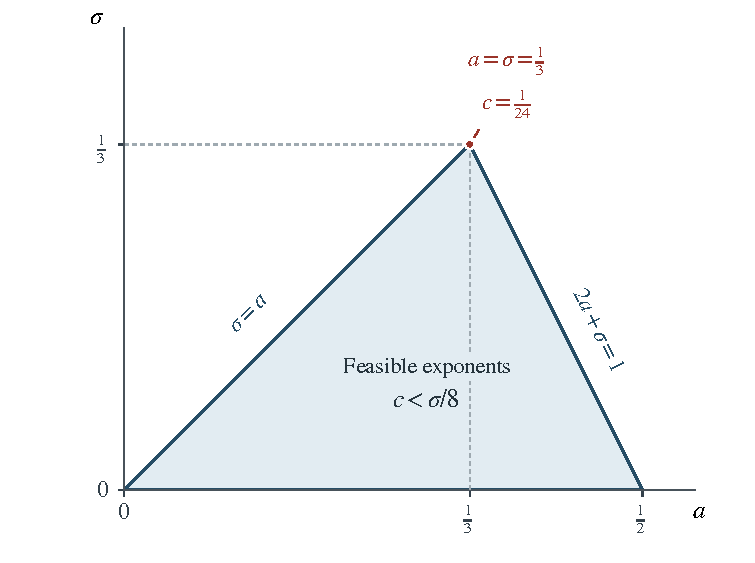
\includegraphics[width=.82\textwidth]{figures/parameter_region.pdf}
 \caption{The closed power-exponent region
 \(0\le\sigma\le a\), \(2a+\sigma\le1\).
 Strict interior choices give the fixed-power construction.
 Logarithmic factors implement the limiting vertex in the endpoint
 theorem. This is the feasible region of the displayed estimates,
 not a lower bound on the complexity of every possible refinement.}
 \label{fig:parameters}
\end{figure}

The logarithmic choices can be understood from the same calculation.
For a small tolerance \(\zeta\), the local-lemma cutoff is of size
\(D\log k/\zeta^2\). The two dominant signature estimates are
of respective sizes
\[
 \frac{D^2\log k}{\zeta^2},
 \qquad \frac{k\log k}{D}.
\]
Equating them suggests \(D\asymp k^{1/3}\zeta^{2/3}\),
and then \(pk\asymp k^{2/3}(\log k)\zeta^{-2/3}\).
Choosing \(\zeta\asymp1/\log k\) keeps the outer-balance loss
of order \(k\) while giving
\[
 \log(1/p)=\tfrac13\log k-\tfrac53\log\log k-O(1).
\]
The binary rich estimate uses approximately
\((k/8)\log(1/p)\) as its size budget, explaining both \(1/24\)
and \(5/24\).
The proofs above establish that these choices work.
They do not establish that either coefficient is an intrinsic
barrier: smaller actual pattern counts, stronger dependence
information, or a different key could change the ledger.

\section{Audit, integration, and further research}
\label{sec:research}

\subsection{Dependency and claim audit}

The proof is finite and self-contained apart from standard real and
integer arithmetic and the finiteness of the usual van der Waerden
numbers used to name \(W_r(k)\). The lower-bound construction itself
does not use a quantitative upper-bound theorem.
The indispensable chain is:
\begin{enumerate}
 \item \Cref{lem:prime-estimates,lem:dilation,lem:mesh} give the
       cyclic coordinates, a controlled dilation, and stable mesh
       neighborhoods.
 \item \Cref{lem:global,lem:local} bound global words and local
       patterns through a specified literal label.
 \item \Cref{prop:outer-tests} applies a finite local lemma to
       distinct-label rows, residual light sets, and local patterns.
 \item \Cref{lem:return,lem:short,thm:dichotomy} convert repeated
       labels into either a global affine lift or near-uniformity.
 \item \Cref{lem:multiplicity,lem:signature,thm:abstract} control
       repeated keys and both kinds of bad event.
 \item \Cref{thm:cyclic} checks every parameter loss, and
       \cref{prop:product,prop:periodic,prop:palette} supply the
       uniform all-color conclusions.
\end{enumerate}

Several mathematical boundaries deserve explicit recording.
The key-count argument uses separation of the actual \(q\)-adic
embedding, not a generic assertion about thin annuli.
The affine event count preserves key identities; a count only up to
renaming keys would be insufficient.
The local lemma uses independent variables attached to labels, while
the final perturbation uses a separate independent family attached to
keys. Independence is never asserted between progressions.
The three-color result controls distance from a constant word and
does not imply occurrence of all three colors.
Finally, the mixed-radix product works even when its moduli share
prime factors, because it uses a divisibility chain, not the Chinese
remainder theorem.

\begin{center}
\small
\begin{tabular}{@{}>{\raggedright\arraybackslash}p{.29\textwidth}>{\raggedright\arraybackslash}p{.27\textwidth}>{\raggedright\arraybackslash}p{.34\textwidth}@{}}
\toprule
Quantity&Displayed source choice&Choice or bound here\\
\midrule
Dimension&\(\cl{k^{1/10}}\)&\(\cl{k^{1/3}(\log k)^{-2/3}}\)\\
Small-prime cutoff&\(D^2\)&\(\cl{AD(\log k)^3}\)\\
Outer binary balance&at least \(k/100\) of each&at least
\((1/2-4/\log k)k\) of each, or affine\\
Key multiplicity&at most four&at most two\\
Perturbation probability&\(k^{-1/20}\)&
\(Bk^{-1/3}(\log k)^{5/3}\)\\
Binary \(k\log k\) coefficient&\(10^{-5}\)&\(1/24\)\\
Color products&binary digits&optimized binary and ternary digits\\
Distance guarantee&nonmonochromatic&order
\(k^{2/3}(\log k)^{5/3}\)\\
\bottomrule
\end{tabular}
\end{center}

\subsection{What the companion computation establishes}

The accompanying \texttt{verify.py} uses exact rational arithmetic for
the palette and probability checks. It verifies the two coefficient
cancellations in \eqref{eq:cancellations}, the correction polynomials
in \eqref{eq:reversion}, the palette optimization over a finite
validation range, and exact mixed-radix floor identities for small
noncoprime and mixed bases. It also checks finite increment spaces
against the rich-event estimate with repeated keys, including
incompatible prescriptions. Its report records the ranges and counts.

These checks are useful for catching algebra, ceiling, carry, and
shared-variable errors. They do not numerically construct the enormous
colorings at the eventual threshold or validate an infinite theorem
by enumeration. The proofs above, including the asymptotic domination
estimates and the local lemma, are the mathematical justification.
The figure is generated from the exact linear inequalities
\eqref{eq:power-ledger}, not from experimental estimates of
van der Waerden numbers.

\subsection{Suggested placement and formalization route}

This package is intended for a distinct research subdirectory under
\texttt{Combinatorics/}\allowbreak\texttt{Ramsey/}\allowbreak\texttt{Research/},
since its new claims are lower
bounds and robustness properties, rather than exact replacements of
the Gowers upper-bound interfaces.
It need not alter the existing 120-statement Gowers ledger.
The source citations are pinned in \texttt{SOURCE\_PROVENANCE.json};
the new article, bibliography, verification program, figure, and build
instructions form a standalone package.

A formalization can be staged at precise mathematical boundaries:
\begin{enumerate}
 \item Prove the norm-band lemma for finite separated subsets of a
       real affine line and then apply the cyclic coordinate
       separation lemma.
 \item Formalize \cref{thm:abstract} for a finite indexed family of
       configurations. This part is independent of the torus meshes.
 \item Formalize the mixed-radix transfer and the exact integer
       palette formula. These are likewise independent of the
       asymptotic analytic estimates.
 \item Formalize mesh-width and neighborhood estimates, arrangement
       sign counts including equality, and the amended residual
       event family.
 \item Assemble the return dichotomy and the endpoint domination
       inequalities, with constants fixed in the stated order.
\end{enumerate}
The new statements should acquire formal status only after those proofs
are actually checked in the selected prover. The existing source's
formalized coefficient \(10^{-5}\) does not transfer formal status to
coefficient \(1/24\) by citation.

\subsection{Further research questions}

\begin{question}[Reduce global label entropy]\label{q:global}
Can the actual global words of the \(q\)-adic embedding be counted
more efficiently than by treating all scalar starts and steps
independently?
\end{question}

The proof currently pays \(D\log\lambda\), of size
\(D^2\) times logarithmic factors.
The scalar homomorphisms are strongly dependent, so their independent
product count may be wasteful.
For orientation, if a valid replacement gave a power-scale cost
\(D^u\), while leaving the quadratic cost \(k/D\) and other steps
intact, the same exponent calculation would permit a binary
coefficient approaching \(1/[8(u+1)]\).
This conditional calculation identifies what an improved count would
buy; it does not supply the count.
Conditioning the word count on a closest return or on a common
carry pattern is a concrete first direction.

\begin{question}[Exploit repeated-key structure]\label{q:keys}
Do nonaffine progressions with many double keys necessarily have
smaller signature complexity, or many incompatible outer-color
prescriptions?
\end{question}

The general two-point geometric bound is best possible, but the final
union bound uses it in every rich progression.
A double key requires the corresponding line segment to meet opposite
sides of a norm minimum. A structural theorem making extensive pairing
either compressible or incompatible with the desired target color
could increase the forced-increment count without changing the mesh.
Proving an average statement is insufficient unless it controls all
remaining bad events.

\begin{question}[Improve the logarithmic correction]\label{q:log}
Can the coefficient \(5/24\) of \(k\log\log k\) in the binary bound
be reduced while retaining the leading coefficient \(1/24\)?
\end{question}

The present value comes from the anchored count, a shrinking balance
tolerance, and the two signature bounds.
A sharper treatment of local dependencies or an entropy bound using
the distribution of anchor widths may change it.
The optimization discussion establishes neither a lower bound on
actual entropy nor a universal second-order obstruction.

\begin{question}[A larger robustness scale]\label{q:robust}
Can one obtain \(N\ge\exp(c k\log k)\), with fixed \(c>0\), while
forcing every \(k\)-term progression to contain a fixed positive
fraction of both colors?
\end{question}

The fixed-power result \cref{thm:tradeoff} reaches every
\(k^\theta\), \(2/3<\theta<1\), at the price of a smaller coefficient,
but its permitted \(c\) tends to zero as \(\theta\to1\).
The endpoint result attains the largest coefficient supported by the
current ledger and a logarithmic enhancement of \(k^{2/3}\).
Whether this tradeoff reflects the problem or just the perturbation
method is not settled by the report.

\begin{question}[Construct and certify the succinct tables]\label{q:algorithm}
Can successful tables from \cref{cor:description} be found and
certified in time polynomial in their description length?
\end{question}

An outer local-lemma algorithm is only part of the task.
The eligible patterns must be enumerated or separated effectively,
and the rich progression failures in the second stage must also be
controlled.
An acceptable certificate should establish coverage of every
configuration rather than merely test a large random sample.
The algebraic form of the mesh endpoints makes exact comparisons
possible, so the problem is combinatorial and quantitative, not an
obstruction from noncomputable real parameters.

\begin{question}[Explicit onset and finite constructions]\label{q:onset}
What explicit numerical constants and onset can be extracted, and
which simplifications help at feasible values of \(k\)?
\end{question}

The current proof deliberately separates existence from numerical
optimization. Tracking an explicit arrangement constant, local
incident weight, and prime-count constant would give an effective
but potentially enormous threshold.
Such a calculation should be compared with direct finite coloring
constructions; the large asymptotic coefficient alone is not evidence
of a better small-\(k\) record.

\begin{question}[Asymmetric progression lengths]\label{q:offdiag}
Can the balanced-or-affine construction be optimized when different
colors forbid different progression lengths?
\end{question}

Biased outer color probabilities and nonuniform increment probabilities
would lead to a multiobjective version of
\cref{thm:abstract}.
The central issue is that the geometric period and mesh parameters
would need to handle several lengths simultaneously.
An exact asymmetric optimization should distinguish a color's
extinction event from proximity to a constant word, a distinction
already essential in the ternary case here.

\begin{question}[Other arithmetic configuration families]\label{q:patterns}
Which systems beyond linear progressions admit simultaneously
bounded key multiplicity and a small literal exceptional-signature
space?
\end{question}

\Cref{thm:abstract} already applies to arbitrary finite configuration
families once those two inputs are supplied.
For polynomial configurations a norm evaluated along the lifted path
has higher degree, but a degree bound by itself does not supply the
separation geometry used in \cref{lem:multiplicity}.
A valid extension must prove the new geometric multiplicity lemma,
rather than assume that the line argument transfers.

\begin{question}[Compare small- and large-palette methods]\label{q:palettes}
Can the present small-palette construction be combined with the
Fox--Hunter shifted-product method to improve the transition where
the number of colors is polylogarithmic in \(k\)?
\end{question}

The direct binary--ternary product loses efficiency as a function of
\(\log r\), whereas Fox--Hunter is substantially stronger once its
large-palette hypothesis holds.
A useful combination would need to preserve quantitative defect
information through each shifted product, with every density loss
recorded. The robust cyclic theorem supplies such an input, but no
improvement in that transition regime is claimed here.

\begin{question}[Kernel-checked constants and proof interfaces]
\label{q:formal}
Can the strengthened finite interfaces, their asymptotic assembly,
and the explicit exponent \(1/24\) be formalized without importing
the stronger endpoint as an assumption?
\end{question}

The return argument, residual-set definition, and shared-key random
variables make useful audit targets.
Their exact quantifiers are more informative than a theorem wrapper
asserting only the final existence of constants.
A successful formalization would both verify this report and provide
reusable lower-bound interfaces beside ProveIt's existing
upper-bound formalization program.

\subsection{Scope of the outcome}

The report proves a substantial quantitative refinement of the selected
repository construction, with an explicit leading coefficient,
logarithmic correction, robustness guarantee, inverse form, and exact
palette optimization.
It does not determine the true asymptotic growth of \(W_2(k)\), prove
optimality of the new constants, claim the best estimate for every
color regime, or provide a formalized proof of the strengthened
theorems. Those boundaries specify what the next research and
verification steps must address.

\clearpage
\bibliographystyle{plain}
\bibliography{references}
\end{document}
